\chapter{Analyse}
Il faut détailler le context du projet, les besoins, les spécifications, etc.

Quelle est la motivation derrière ce projet ? Qu'est-ce que ce projet apportera au final ?

On peut rajouter un diagramme WBS pour donner un aperçu haut-niveau :
\begin{figure}[h]
    \centering
    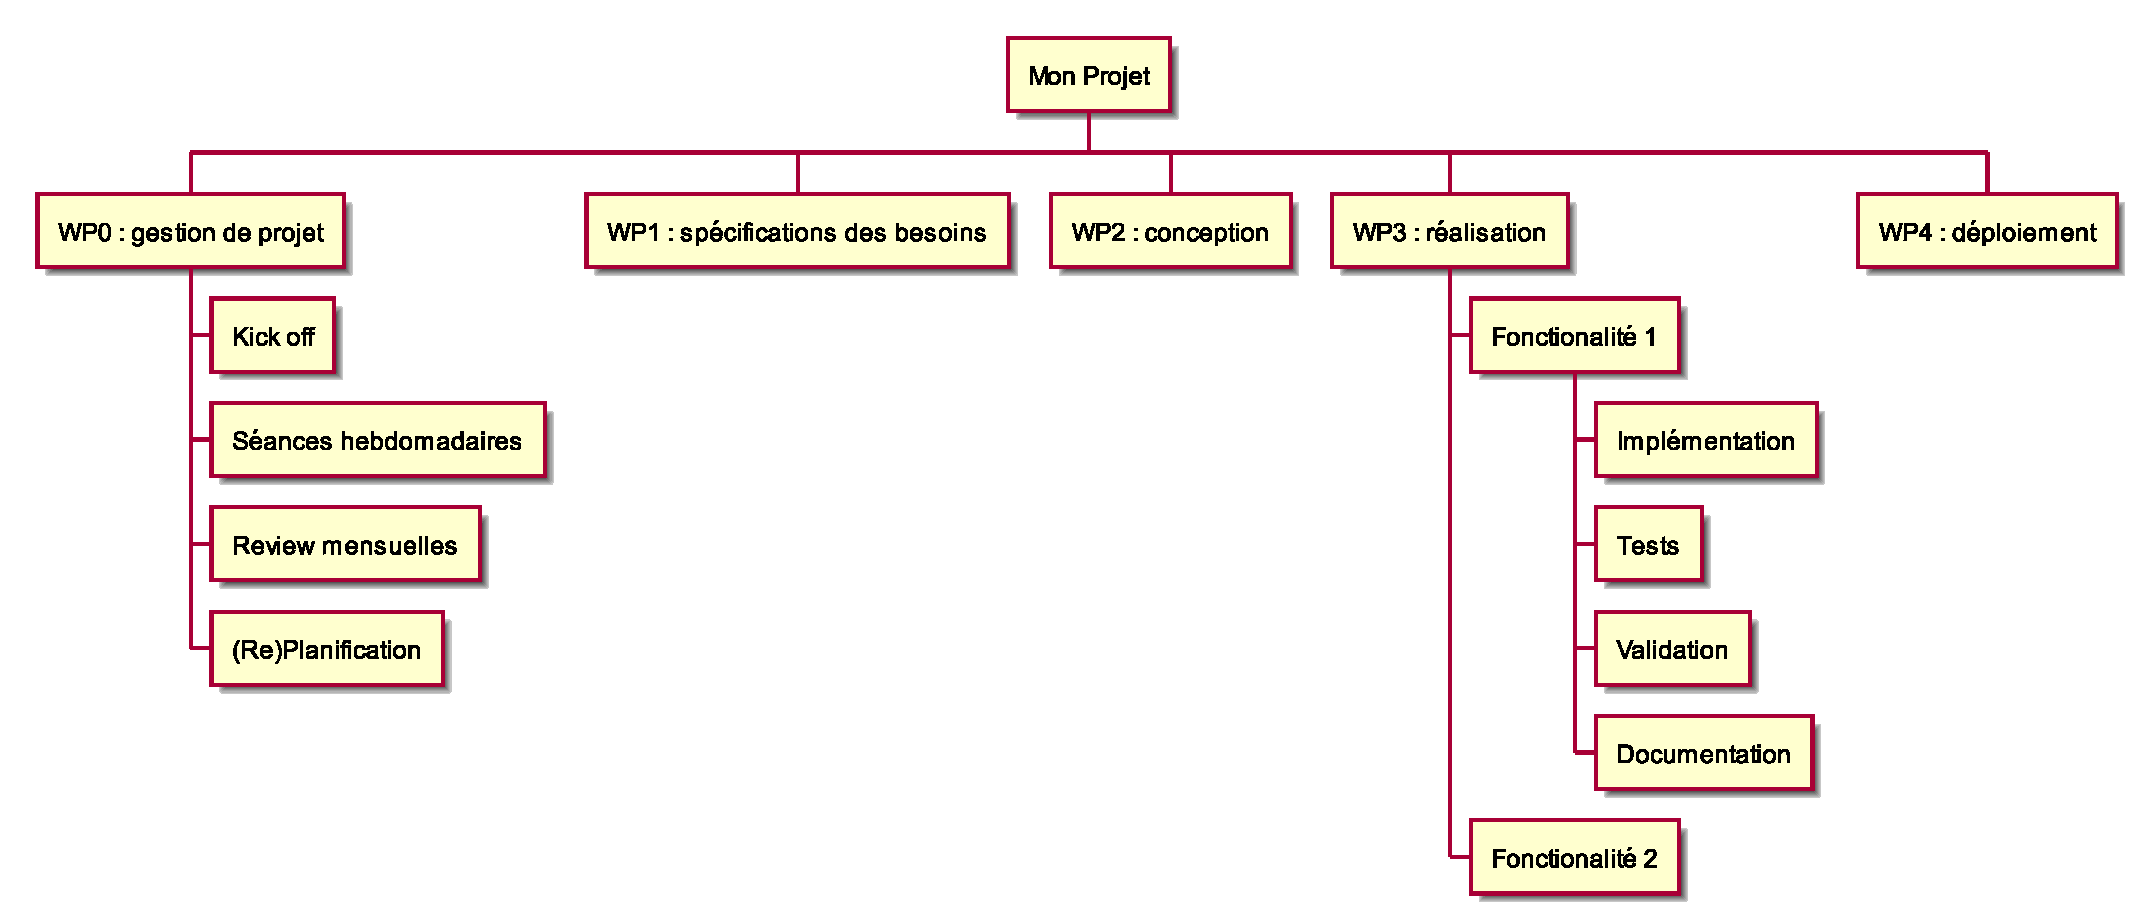
\includegraphics[width=\textwidth]{./images/WBS_Exemple.eps}
    \caption{Diagramme WBS qui va bien.}
\end{figure}

\section{Faisabilité}
Quels sont les contraintes de ce projet ? En quoi elles sont surmontables ? Un preuve de concept existe-t'elle déjà ?

\section{Risques}
Faire une analyse de risques et donner les solutions envisagées le cas échéant.
Pour chaque risque, il faut détailler les informations suivantes :
\begin{itemize}
  \item Son numéro;
  \item Son nom;
  \item Sa description;
  \item Sa probabilité : très improbable, improbable, probable, très probable;
  \item Son impact :  faible, modéré, grave, très grave;
  \item Niveau de criticité (Probabilité * Impact)
  \item Les mesures de prévention
  \item Les mesure de correction
\end{itemize}

Ensuite, on peut résumer ces informations dans un tableau comme ce qui suit :

\begin{tabular}{ | l | l | l | l | }
  N° & Nom & Probabilité & Impact \\
  \rowcolor{red!60}
  01 & Risque critique & probable & grave \\
  \rowcolor{red!20}
  02 & Risque acceptable & probable & faible \\
  03 & Risque insignifiant & peu probable & faible
\end{tabular}

\section{Planification}
Il faut rajouter un diagramme de Gantt ici.

\section{Technologies utilisées}
Expliquer les choix concernant les technologies.
Si possible, montrer les avantages et les inconvénients de chaque technologie pour justifier ses choix.
Si un prototype est créé pour tester des points chauds, c'est intéressant de le mentionner ici.
